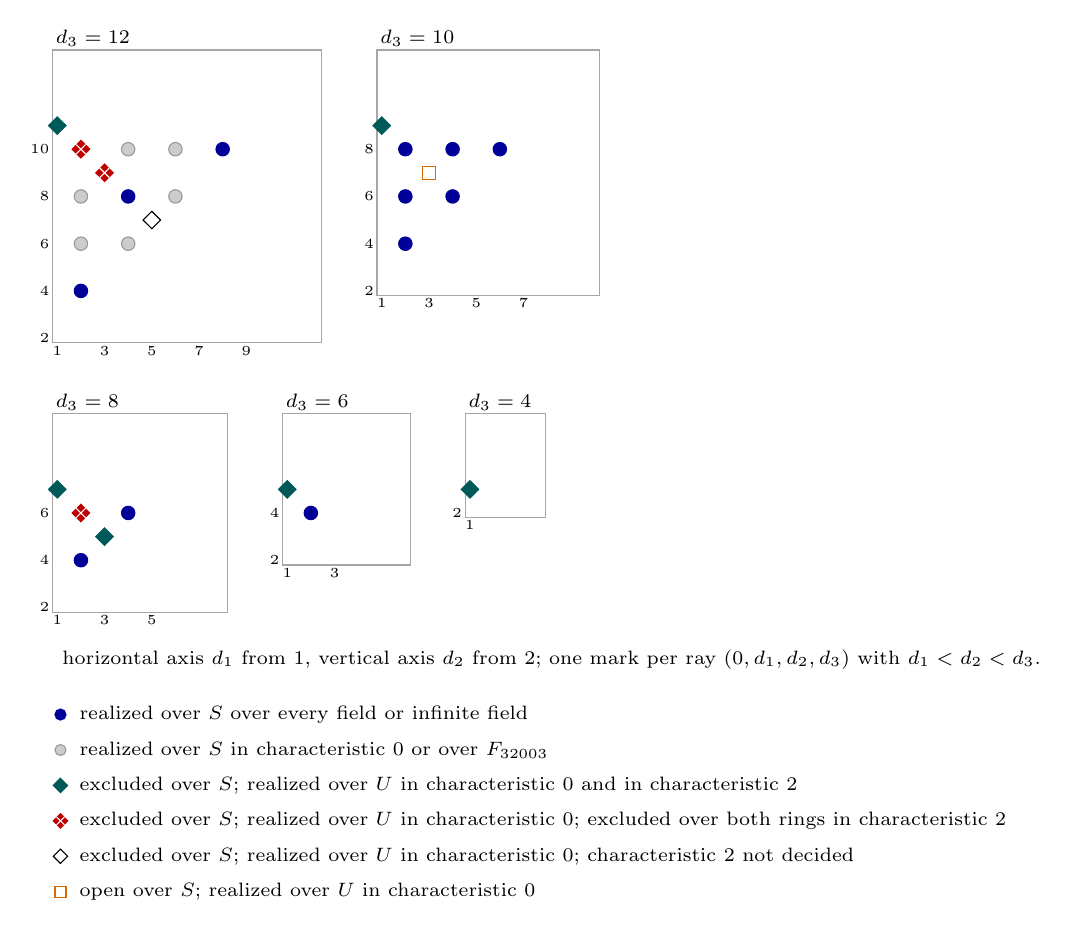
\begin{tikzpicture}[x=1cm,y=1cm,font=\scriptsize]
\begin{scope}[shift={(0.000,-3.720)}]
\draw[gray!70, line width=0.4pt] (0,0) rectangle (3.420,3.720);
\node[anchor=south west,inner sep=1pt] at (0,3.720) {$d_3=12$};
\node[anchor=north,inner sep=1pt,font=\tiny] at (0.060,0) {1};
\node[anchor=north,inner sep=1pt,font=\tiny] at (0.660,0) {3};
\node[anchor=north,inner sep=1pt,font=\tiny] at (1.260,0) {5};
\node[anchor=north,inner sep=1pt,font=\tiny] at (1.860,0) {7};
\node[anchor=north,inner sep=1pt,font=\tiny] at (2.460,0) {9};
\node[anchor=east,inner sep=1pt,font=\tiny] at (0,0.060) {2};
\node[anchor=east,inner sep=1pt,font=\tiny] at (0,0.660) {4};
\node[anchor=east,inner sep=1pt,font=\tiny] at (0,1.260) {6};
\node[anchor=east,inner sep=1pt,font=\tiny] at (0,1.860) {8};
\node[anchor=east,inner sep=1pt,font=\tiny] at (0,2.460) {10};
\draw[teal!70!black, fill=teal!70!black, line width=0.4pt] (-0.051,2.760) -- (0.060,2.870) -- (0.171,2.760) -- (0.060,2.649) -- cycle;
\draw[blue!60!black, fill=blue!60!black, line width=0.4pt] (0.360,0.660) circle (0.085);
\draw[gray!80, fill=gray!40, line width=0.4pt] (0.360,1.260) circle (0.085);
\draw[gray!80, fill=gray!40, line width=0.4pt] (0.360,1.860) circle (0.085);
\draw[red!75!black, fill=red!75!black, line width=0.4pt] (0.249,2.460) -- (0.360,2.571) -- (0.471,2.460) -- (0.360,2.349) -- cycle; \draw[white, line width=0.4pt] (0.300,2.401) -- (0.419,2.519) (0.300,2.519) -- (0.419,2.401);
\draw[red!75!black, fill=red!75!black, line width=0.4pt] (0.549,2.160) -- (0.660,2.271) -- (0.770,2.160) -- (0.660,2.050) -- cycle; \draw[white, line width=0.4pt] (0.600,2.101) -- (0.719,2.220) (0.600,2.220) -- (0.719,2.101);
\draw[gray!80, fill=gray!40, line width=0.4pt] (0.960,1.260) circle (0.085);
\draw[blue!60!black, fill=blue!60!black, line width=0.4pt] (0.960,1.860) circle (0.085);
\draw[gray!80, fill=gray!40, line width=0.4pt] (0.960,2.460) circle (0.085);
\draw[black, fill=white, line width=0.4pt] (1.149,1.560) -- (1.260,1.671) -- (1.371,1.560) -- (1.260,1.450) -- cycle;
\draw[gray!80, fill=gray!40, line width=0.4pt] (1.560,1.860) circle (0.085);
\draw[gray!80, fill=gray!40, line width=0.4pt] (1.560,2.460) circle (0.085);
\draw[blue!60!black, fill=blue!60!black, line width=0.4pt] (2.160,2.460) circle (0.085);
\end{scope}
\begin{scope}[shift={(4.120,-3.120)}]
\draw[gray!70, line width=0.4pt] (0,0) rectangle (2.820,3.120);
\node[anchor=south west,inner sep=1pt] at (0,3.120) {$d_3=10$};
\node[anchor=north,inner sep=1pt,font=\tiny] at (0.060,0) {1};
\node[anchor=north,inner sep=1pt,font=\tiny] at (0.660,0) {3};
\node[anchor=north,inner sep=1pt,font=\tiny] at (1.260,0) {5};
\node[anchor=north,inner sep=1pt,font=\tiny] at (1.860,0) {7};
\node[anchor=east,inner sep=1pt,font=\tiny] at (0,0.060) {2};
\node[anchor=east,inner sep=1pt,font=\tiny] at (0,0.660) {4};
\node[anchor=east,inner sep=1pt,font=\tiny] at (0,1.260) {6};
\node[anchor=east,inner sep=1pt,font=\tiny] at (0,1.860) {8};
\draw[teal!70!black, fill=teal!70!black, line width=0.4pt] (-0.051,2.160) -- (0.060,2.271) -- (0.171,2.160) -- (0.060,2.050) -- cycle;
\draw[blue!60!black, fill=blue!60!black, line width=0.4pt] (0.360,0.660) circle (0.085);
\draw[blue!60!black, fill=blue!60!black, line width=0.4pt] (0.360,1.260) circle (0.085);
\draw[blue!60!black, fill=blue!60!black, line width=0.4pt] (0.360,1.860) circle (0.085);
\draw[orange!85!black, fill=white, line width=0.4pt] (0.575,1.475) rectangle (0.745,1.645);
\draw[blue!60!black, fill=blue!60!black, line width=0.4pt] (0.960,1.260) circle (0.085);
\draw[blue!60!black, fill=blue!60!black, line width=0.4pt] (0.960,1.860) circle (0.085);
\draw[blue!60!black, fill=blue!60!black, line width=0.4pt] (1.560,1.860) circle (0.085);
\end{scope}
\begin{scope}[shift={(0.000,-7.140)}]
\draw[gray!70, line width=0.4pt] (0,0) rectangle (2.220,2.520);
\node[anchor=south west,inner sep=1pt] at (0,2.520) {$d_3=8$};
\node[anchor=north,inner sep=1pt,font=\tiny] at (0.060,0) {1};
\node[anchor=north,inner sep=1pt,font=\tiny] at (0.660,0) {3};
\node[anchor=north,inner sep=1pt,font=\tiny] at (1.260,0) {5};
\node[anchor=east,inner sep=1pt,font=\tiny] at (0,0.060) {2};
\node[anchor=east,inner sep=1pt,font=\tiny] at (0,0.660) {4};
\node[anchor=east,inner sep=1pt,font=\tiny] at (0,1.260) {6};
\draw[teal!70!black, fill=teal!70!black, line width=0.4pt] (-0.051,1.560) -- (0.060,1.671) -- (0.171,1.560) -- (0.060,1.450) -- cycle;
\draw[blue!60!black, fill=blue!60!black, line width=0.4pt] (0.360,0.660) circle (0.085);
\draw[red!75!black, fill=red!75!black, line width=0.4pt] (0.249,1.260) -- (0.360,1.371) -- (0.471,1.260) -- (0.360,1.149) -- cycle; \draw[white, line width=0.4pt] (0.300,1.200) -- (0.419,1.320) (0.300,1.320) -- (0.419,1.200);
\draw[teal!70!black, fill=teal!70!black, line width=0.4pt] (0.549,0.960) -- (0.660,1.071) -- (0.770,0.960) -- (0.660,0.849) -- cycle;
\draw[blue!60!black, fill=blue!60!black, line width=0.4pt] (0.960,1.260) circle (0.085);
\end{scope}
\begin{scope}[shift={(2.920,-6.540)}]
\draw[gray!70, line width=0.4pt] (0,0) rectangle (1.620,1.920);
\node[anchor=south west,inner sep=1pt] at (0,1.920) {$d_3=6$};
\node[anchor=north,inner sep=1pt,font=\tiny] at (0.060,0) {1};
\node[anchor=north,inner sep=1pt,font=\tiny] at (0.660,0) {3};
\node[anchor=east,inner sep=1pt,font=\tiny] at (0,0.060) {2};
\node[anchor=east,inner sep=1pt,font=\tiny] at (0,0.660) {4};
\draw[teal!70!black, fill=teal!70!black, line width=0.4pt] (-0.051,0.960) -- (0.060,1.071) -- (0.171,0.960) -- (0.060,0.849) -- cycle;
\draw[blue!60!black, fill=blue!60!black, line width=0.4pt] (0.360,0.660) circle (0.085);
\end{scope}
\begin{scope}[shift={(5.240,-5.940)}]
\draw[gray!70, line width=0.4pt] (0,0) rectangle (1.020,1.320);
\node[anchor=south west,inner sep=1pt] at (0,1.320) {$d_3=4$};
\node[anchor=north,inner sep=1pt,font=\tiny] at (0.060,0) {1};
\node[anchor=east,inner sep=1pt,font=\tiny] at (0,0.060) {2};
\draw[teal!70!black, fill=teal!70!black, line width=0.4pt] (-0.051,0.360) -- (0.060,0.471) -- (0.171,0.360) -- (0.060,0.249) -- cycle;
\end{scope}
\node[anchor=north west,font=\scriptsize] at (0,-7.490) {horizontal axis $d_1$ from 1, vertical axis $d_2$ from 2; one mark per ray $(0,d_1,d_2,d_3)$ with $d_1<d_2<d_3$.};
\draw[blue!60!black, fill=blue!60!black, line width=0.4pt] (0.100,-8.440) circle (0.070);
\node[anchor=west,font=\scriptsize,inner sep=1pt] at (0.30,-8.44) {realized over $S$ over every field or infinite field};
\draw[gray!80, fill=gray!40, line width=0.4pt] (0.100,-8.890) circle (0.070);
\node[anchor=west,font=\scriptsize,inner sep=1pt] at (0.30,-8.89) {realized over $S$ in characteristic 0 or over $\mathbb{F}_{32003}$};
\draw[teal!70!black, fill=teal!70!black, line width=0.4pt] (0.009,-9.340) -- (0.100,-9.249) -- (0.191,-9.340) -- (0.100,-9.431) -- cycle;
\node[anchor=west,font=\scriptsize,inner sep=1pt] at (0.30,-9.34) {excluded over $S$; realized over $U$ in characteristic 0 and in characteristic 2};
\draw[red!75!black, fill=red!75!black, line width=0.4pt] (0.009,-9.790) -- (0.100,-9.699) -- (0.191,-9.790) -- (0.100,-9.881) -- cycle; \draw[white, line width=0.4pt] (0.051,-9.839) -- (0.149,-9.741) (0.051,-9.741) -- (0.149,-9.839);
\node[anchor=west,font=\scriptsize,inner sep=1pt] at (0.30,-9.79) {excluded over $S$; realized over $U$ in characteristic 0; excluded over both rings in characteristic 2};
\draw[black, fill=white, line width=0.4pt] (0.009,-10.240) -- (0.100,-10.149) -- (0.191,-10.240) -- (0.100,-10.331) -- cycle;
\node[anchor=west,font=\scriptsize,inner sep=1pt] at (0.30,-10.24) {excluded over $S$; realized over $U$ in characteristic 0; characteristic 2 not decided};
\draw[orange!85!black, fill=white, line width=0.4pt] (0.030,-10.760) rectangle (0.170,-10.620);
\node[anchor=west,font=\scriptsize,inner sep=1pt] at (0.30,-10.69) {open over $S$; realized over $U$ in characteristic 0};
\end{tikzpicture}
